\documentclass{hotnets21}

\usepackage{times}  
\usepackage{hyperref}
\usepackage{titlesec}
\usepackage{graphicx}

\graphicspath{ {../results/US/} }

\hypersetup{pdfstartview=FitH,pdfpagelayout=SinglePage}

\setlength\paperheight {11in}
\setlength\paperwidth {8.5in}
\setlength{\textwidth}{7in}
\setlength{\textheight}{9.25in}
\setlength{\oddsidemargin}{-.25in}
\setlength{\evensidemargin}{-.25in}

\newcommand{\dotgov}{\textit{.gov}\space}
\newcommand{\csv}{csv\space}

% Some data which will need to be copied before we submit
\newcommand{\foreignmslocations}{19\space}

\begin{document}

% \conferenceinfo{HotNets 2021} {}
\CopyrightYear{2024}
% \crdata{X}
\date{3/14/2024}

%%%%%%%%%%%% THIS IS WHERE WE PUT IN THE TITLE AND AUTHORS %%%%%%%%%%%%

\title{Where is Your Mail? Analysis of US Government Domain Mail Server Geolocation}

\author{Kevin Hayes, Jay Park, Hong Zhou}

\maketitle

%%%%%%%%%%%%%  ABSTRACT GOES HERE %%%%%%%%%%%%%%
\begin{abstract}

Electronic communication is ubiquitous across personal, industrial, and government circles.
Indeed, as the prevalence of tools such as instant messaging, online chats and, in particular, emails continues to grow globally, so does the incentive of third parties to tamper and surveil the sensitive information transmitted across the modern internet.
With rising political interest in cybersecurity - particularly cyber attacks - and each government’s interest in data security and sovereignty, we seek to partially address the issue of mail server security in known government domains.
Works in this and adjacent fields have been published in the recent past, with~\cite{bartoli} analyzing the roles network architecture and Route Origin Access plays in mail server security.
To put these previous findings in a real world context, we geolocated a numerous list of mail server IP addresses found through DNS queries on the country-level.
We then mapped the IP addresses with their country of use and the geolocated nation.

\end{abstract}

\section{Introduction}

Over the past decade, communication over the internet has become crucial for both personal and professional communication.
Email in particular is used everyday to convey private information that could be potentially sensitive for one or more parties.
As such, the security of the networks on which these systems relay data is of utmost importance to most major players of the internet.
One such prevalent party with interest at stake is the U.S. Government.

As the government places more emphasis on online services, especially due to the COVID-19 pandemic, the trustworthiness of emails from government domains is extremely important for citizens.
This increased importance also makes government email servers a crucial part of national security and a clear target for attack.
As such, whether or not the email infrastructure of one’s government is trustworthy is important, either in order to provide peace of mind when interacting with government organizations over email, or to caution citizens when receiving emails from government domains.

In this paper, we aim to characterize the present usage of mail servers by United States governments.
This is done by measuring factors such as the configuration of the mail servers, the redundancy/overlap of servers across different domains, and how extensive the use of third-party servers is by \dotgov domains.
This is all done with an emphasis on how the different levels of government manage their infrastructure differently, from city governments to the federal branches. as well as the physical locations which mail servers are located.

We perform DNS lookups on numerous \dotgov domains to extract their associated mail servers and their IP addresses.
In order to find where the mail servers are located, we use IPInfo to map IPs to geolocations. If the analysis shows that the mail server is located in a foreign country, it could be cause for concern.

\section{Contributions}

Our main contributions in this study are as follows:
\begin{itemize}
\item
Using geolocation to gain preliminary understanding of the physical security of government mail servers.
In this area, we found that while the majority of mail server locations used by \dotgov domains reside within the borders of the United States, a small percentage are being hosted outside of the country.
\item
An analysis of the prevalence of first and third-parties in mail servers and their physical locations. Verifying previous studies, and making new contributions by determining how the different levels of government treat third party providers differently.
\item
Measuring the redundancy in mail servers used by \dotgov domains as well as the centralization of mail servers to determine the reliability/vulnerability of government services.
\end{itemize}

\section{Background}

\subsection{Mail Servers}

In order to enable e-mail services for a domain, the owner of a domain must add DNS MX record(s) to the set of records for their domain.
Each of these records contains an \textit{exchange} field, which contains a domain name, corresponding to a mail server which is responsible for sending and receiving mail on the behalf of the domain.
In this paper we will refer to these servers as \textit{mail servers}. A single domain can be served by multiple mail servers, either by listing multiple MX records, each with a different domain.
Or through other load balancing techniques such as mapping multiple IP's to a single mail server domain, or even by mapping multiple servers to a single IP by utilizing IP anycast.
In practice though we've found simply listing multiple MX records to be the most common approach used.

In order to differentiate between these different mail server domains, MX records contain an extra \textit{preference} field, which is a single number used to indicate the order in which mail servers should be contacted.
For example, if \textit{cia.gov} contains two MX records, one for \textit{mail0.outlook.com} with preference 10, and another for \textit{mail1.outlook.com} with preference 20, then when sending mail to a CIA email account, one should first try to connect to \textit{mail0.outlook.com}.
And then only resort to using \textit{mail1.outlook.com} if the first server is unresponsive, because the first server has a lower preference number, and thus a higher priority.

\subsection{Prior Work}

Studies have been done on mail domain zones as well as the zones containing mail servers for said mail domain (referred to as Direct Zones).
Specifically, research on the security of mail servers used by various countries has been done by studying these direct zones, such as the path redundancies of the mail servers, the DNS redundancies for each zone, mail server redundancy, etc.
Current studies also examine the existence of “Route Origin Authorization” in the mail domain level, network level, and AS level.
However, existing research limits their direct zones only to network and Autonomous Systems.

Because previous work has shown the trend among government organizations to utilize mail providers, we’d like to determine where these mail servers are physically located.
Effectively answering the question of “where’s your mail” to go alongside “who’s got your mail” question posed by~\cite{liu}.
If these servers are located in a foreign country, that creates a concern for the security of the servers.

\cite{liu}~also introduces a methodology for determining the mail provider from a given domain, and applies that methodology to the U.S. government’s \dotgov domains, in order to examine the use of third party email providers by different branches of the U.S. government.
We make a slight modification to that approach so that it better serves our interests.

\section{Methodology}

\subsection{Data Sets}
For each domain in our set of government domains~\cite{cisadomains}, we first run DNS queries to obtain the MX records of that domain, creating a map from government domain to mail server domain.
Then we can take those records and run another set of queries to get the IP addresses associated which each mail domain through DNS A records.

This process is relatively straightforward, and we have scripted the entire process, from a list of domains, to running a set of analyses on the final data, using python.
The code and final set of data and graphs can be found at~\cite{ourgithubrepo}~in order to faciliate reproducibility and possibly facilitate future analysis of governments other than the U.S.

Once we have our final mapping from government domain to mail server(s) and corresponding IP(s), we then we then can take the set of IP addresses and cross reference them against two different datasets to determine their geographic and network information.

\subsection{Geolocation}

First we reference each mail server IP against the IPInfo~\cite{ipinfo}~geo location service's database.
This gives us a wide range of information about the physical location of the IP, ranging from broad classifications such as which country the IP is thought to be in, to a specific longitude and latitude point on the globe.
When determining a \textit{location} in the analysis of the data, we are referring to a specific pair of latitude and longitude, because of the wide range of detail levels in the IPInfo dataset.

There are pros and cons to this approach of determining locations, but in general we believe it should be relatively unbiased, because it can both over and under count in different situations.
For example, if two servers are located in different regions of the same state, but IPInfo does not have any more information than the state, then they will both be mapped to the center point of the state, and considered to be the same location, thus an undercount.
However if two servers are truly co-located, but IPInfo has a different levels of detail for each, then we would not be able to tell the difference, for example, if one is mapped to the center of the state, and the other is mapped to the center of the specific city.

\subsection{ASN's and IP Anycast}

The IPInfo dataset also contains entries indicating the Autonomous System Number associated with the IP and whether or not it is an anycast IP.
We do utilize IPInfo for analysis related to IP anycast, though we refer to a more reliable CAIDA dataset~\cite{caidaiptoasn}~for mapping IP's to specific ASN's.
We are unsure how reliable the IPInfo dataset is for determining anycast IP's, and in the future would like to use a dataset specifically for anycast.

\subsection{Mail Server Preferences}

Because we query for all MX records of each domain, we can determine the realtive "rank" of each mail server from the perspective of each domain.
We do this in order to determine how complex the policies behind domains with multiple MX servers.
If we see a wide range of perferences, then that indicates that there is a large number of "backup" mail servers, which are not being used normally.
Or if most servers are ranked similarly, and are thus used more or less equally.
This also serves as an indication for the importance of each mail server from the perspective of the government domain, and restrict some analysis to only servers which are ranked higher.

\subsection{Third Party Mail Servers}

Finally, we measure the usage of third party mail servers, as opposed to the government using their own servers to facilitate mail transfer.
We used an extremely coarse method for determining third party servers, analyzing the mail domain name itself, and classifying each mail domain as either, first party, third party, or unknown.

We use a set of regular expressions trying to match common third party mail providers domain names to each server.
And concluding it's a third party if we find a match.
If we cannot find a match, we then check to see if the domain is itself within the top level \dotgov domain, and if we conclude it is a first party server, hosted by the US government.
If both methods fail, then we mark the mail domain as "unknown".

This method has major drawbacks: the third party analysis would not be comprehensive, as our hard-coded list of third parties would not be exhaustive.
And it makes the task of associating servers with a specific company more difficult, as each rule needs to be manually created, and checked to make sure it is owned by the correct company.
It also does not allow us to conclude which entity within the \dotgov domain is hosting the server. So it is possible that one part of the U.S. government is hosting a mail server for another, and hence not truly a first party server.

However, despite these drawbacks, we were able to classify upwards of 80\% of domains, so we chose to use this relatively simple approach.

An arguably better, though more complicated, method is instead to utilize an IP to ASN mapping, and then using WHOIS queries to determine which entity owns the specific ASN.
We can check if a third-party provider is being used if the ASN does not belong to the US Government and concretely confirm the identity of the third party itself.
This approach assumes that the owner of the mail server also owns the AS which the server is located within, which may not be true, especially for lower levels of goverment such as smaller cities and counties.
In the future we would like to utilize a combination of domain name analysis and ASN ownership to make our determination.

\section{Results}

\subsection{Mail Server Locations}

We can see the distributions of mail server country in Figure \ref{fig:countrysummary} as a log scale.
As might be expected, the vast majority of mail servers’ locations are found are within the United States, with 495 unique domestic locations, and only 19 foreign locations.
We can see that most of these foreign locations are in US-friendly countries, notably Canada, Denmark, France, the Netherlands, and Hong Kong.

\begin{figure}
\label{fig:countrysummary}
\noindent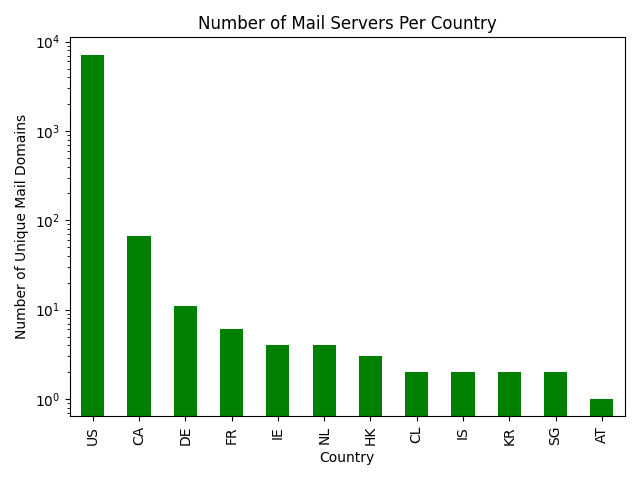
\includegraphics[width=0.5\textwidth]{Summary/Exchanges Per Country Counts.png}
\caption{Mail Server Domains Per Country}
\end{figure}

At first we hypothesized that these foreign locations would be hosted by the state department, or US embassies abroad.
Yet somewhat surprisingly we found that when we associated the foreign locations with a level of government as seen in Figure \ref{fig:globesummary}, then most of the locations abroad are hosted at a lower level of government, at the city or county level.
And we found that the national branches of government were almost entirely hosted within the US.
This makes sense in retrospect, because of the increased importance of security at the natinal level, which means they are more likely to host servers domestically.
Whereas a local government is less concerned with security from foreign governments, and is more likely to use a thrid party provider which may use foreign servers.

\begin{figure}
\label{fig:globesummary}
\noindent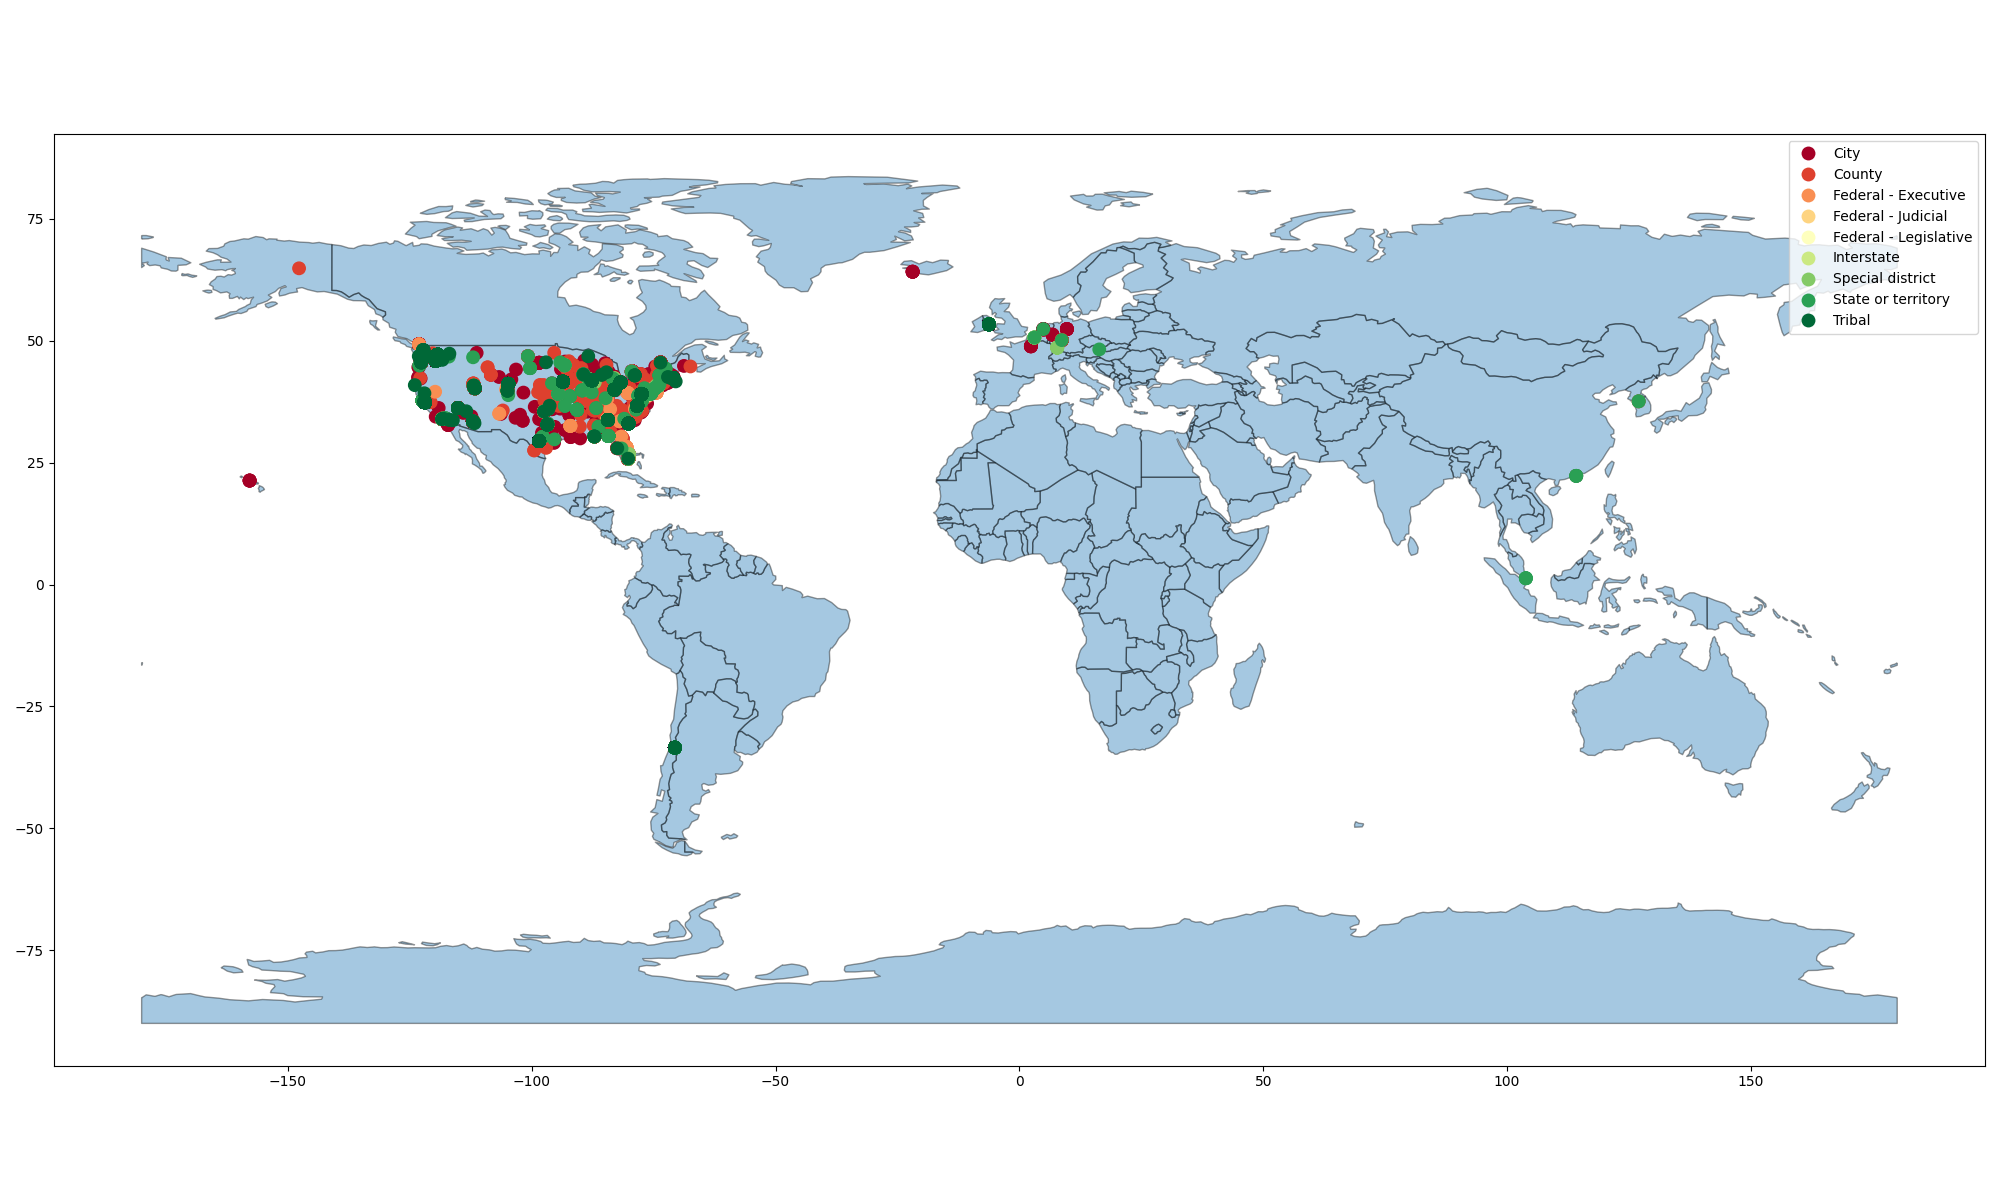
\includegraphics[width=0.5\textwidth]{Summary/Globe.png}
\caption{US Government Mail Server Locations}
\end{figure}

\subsection{IP Anycast}

Surprisingly, we found a number of mail server addresses, 254 total, which were flagged by IPInfo as being IP anycast addresses.
Through anycast, a single domain could potentially use MX exchanges in multiple locations with the same IP, which we would not be able to detect.
Most of these locations were within the US, particularly in cities, such as San Francisco, Seattle, Kansas City, San Antonio, and Jacksonville.

\subsection{Mail Server Preferences}

After ranking the MX records of every \dotgov domain, where servers with the same preference level receive the same ranking, we can observe that the vast majority of records are ranked equally.
Figure \ref{fig:preferenceus} shows domestic locations mapped by preference, with redder points indicating a more prefered server.
This illustratively captures the fact that most domains are given very high rankings, with only a very small number of government domains creating a wide range of preferences.

This trend continues when considering the entire globe, with foreign and domestic locations not having a significant difference in preference levels, and across different levels of government.

\begin{figure}
\label{fig:preferenceus}
\noindent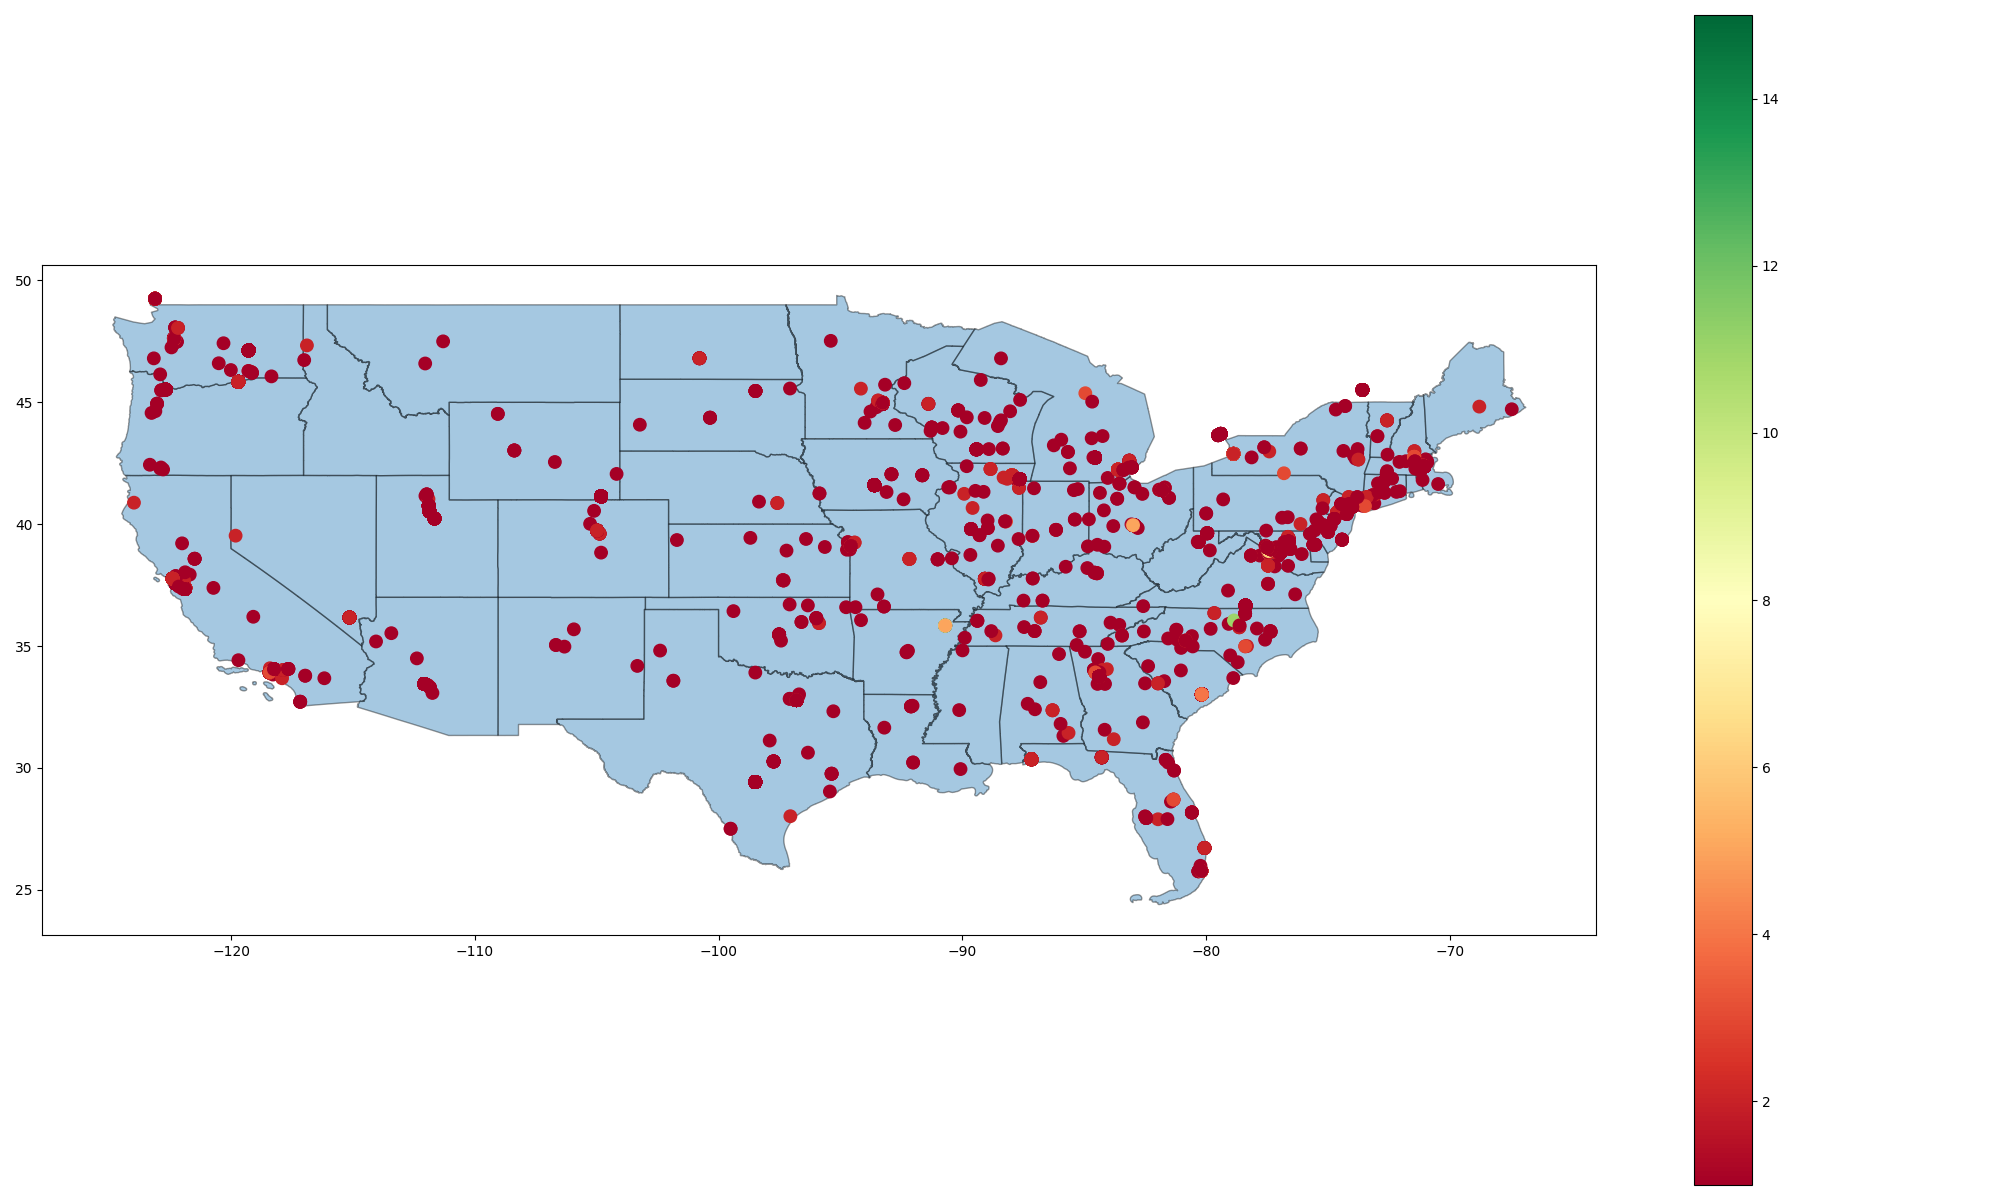
\includegraphics[width=0.5\textwidth]{Summary/US Preference.png}
\caption{Mail Server Preference Rankings}
\end{figure}

\subsection{Mail Server Centralization}

We created a CDF of the number of physical locations a single \dotgov domain has listed as a mail exchange.
We see that 11\% of \dotgov domains were mapped to a single physical server, while the remaining 88\% map to at least 2 physical locations.
We also see that the most prevalent number of locations used is 4 locations, followed by 7 locations.
This shows that most \dotgov domains have redundant systems, which is good for reliability.

\begin{figure}
\label{fig:locationcdf}
\noindent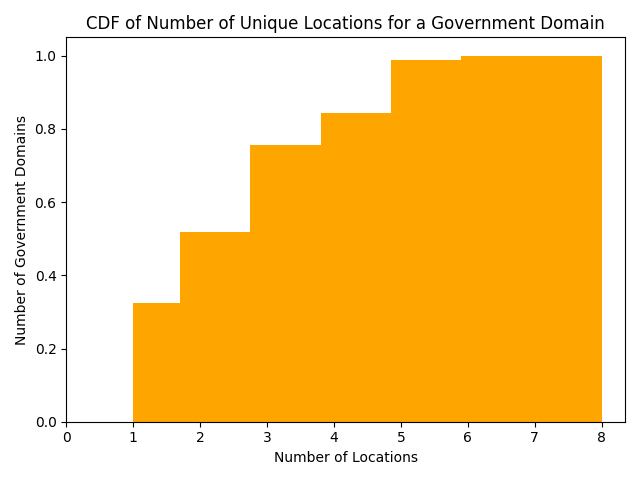
\includegraphics[width=0.5\textwidth]{Summary/Location Count CDF.png}
\caption{CDF of Unqiue Mail Server Locations}
\end{figure}

\begin{figure}
\label{fig:asncdf}
\noindent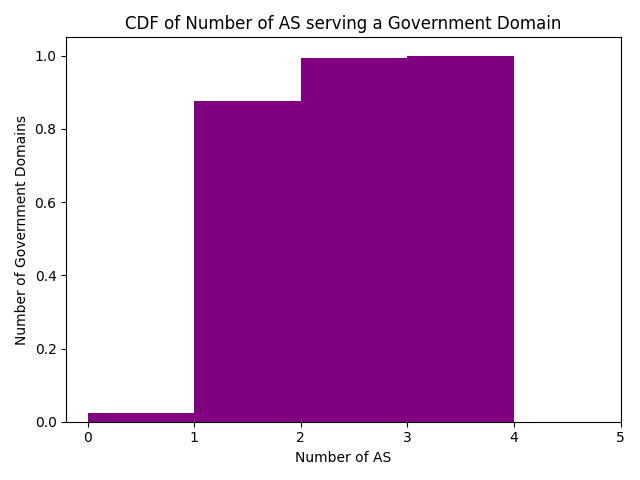
\includegraphics[width=0.5\textwidth]{Summary/ASN Count CDF.png}
\caption{CDF of Unqiue Mail Server AS Number}
\end{figure}

\subsection{Third Party Mail Servers}

Even using our simplified domain name analysis, we are able to classify approximately 89\% of mail server domains as either First or Third party.
And as can be seen in Figure \ref{fig:thirdpartysummary}, 85\% of domains are detected as thrid party, and only 4.5\% are able to be classified as first party.
With the remaining 10.5\% being unknown.

\begin{figure}
\label{fig:thirdpartysummary}
\noindent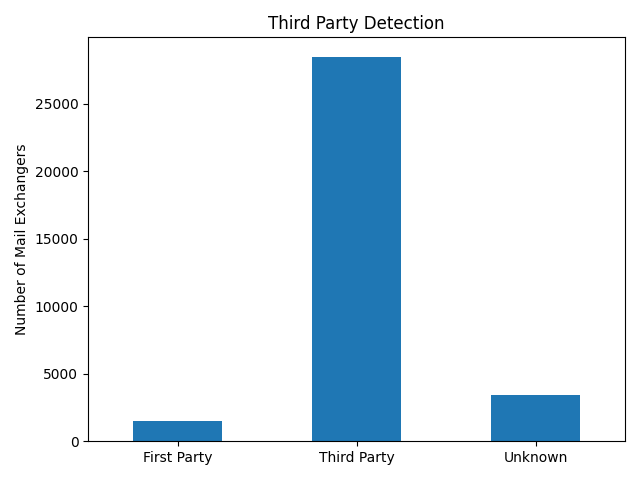
\includegraphics[width=0.5\textwidth]{Summary/Third Party Exchanges.png}
\caption{First, Third, and Unknown Party Mail Server Counts}
\end{figure}

Seeing the distribution of these third party locations on the globe in Figure \ref{fig:thirdpartyglobe}, we can see that every mail domain which we can confidently classify as first party, is located within the borders of the United States.
And many of the foreign locations we discovered we can confidently conclude are third party servers, being hosted in data centers owned by companies such as Microsoft, Google, and Amazon.

\begin{figure}
\label{fig:thirdpartyglobe}
\noindent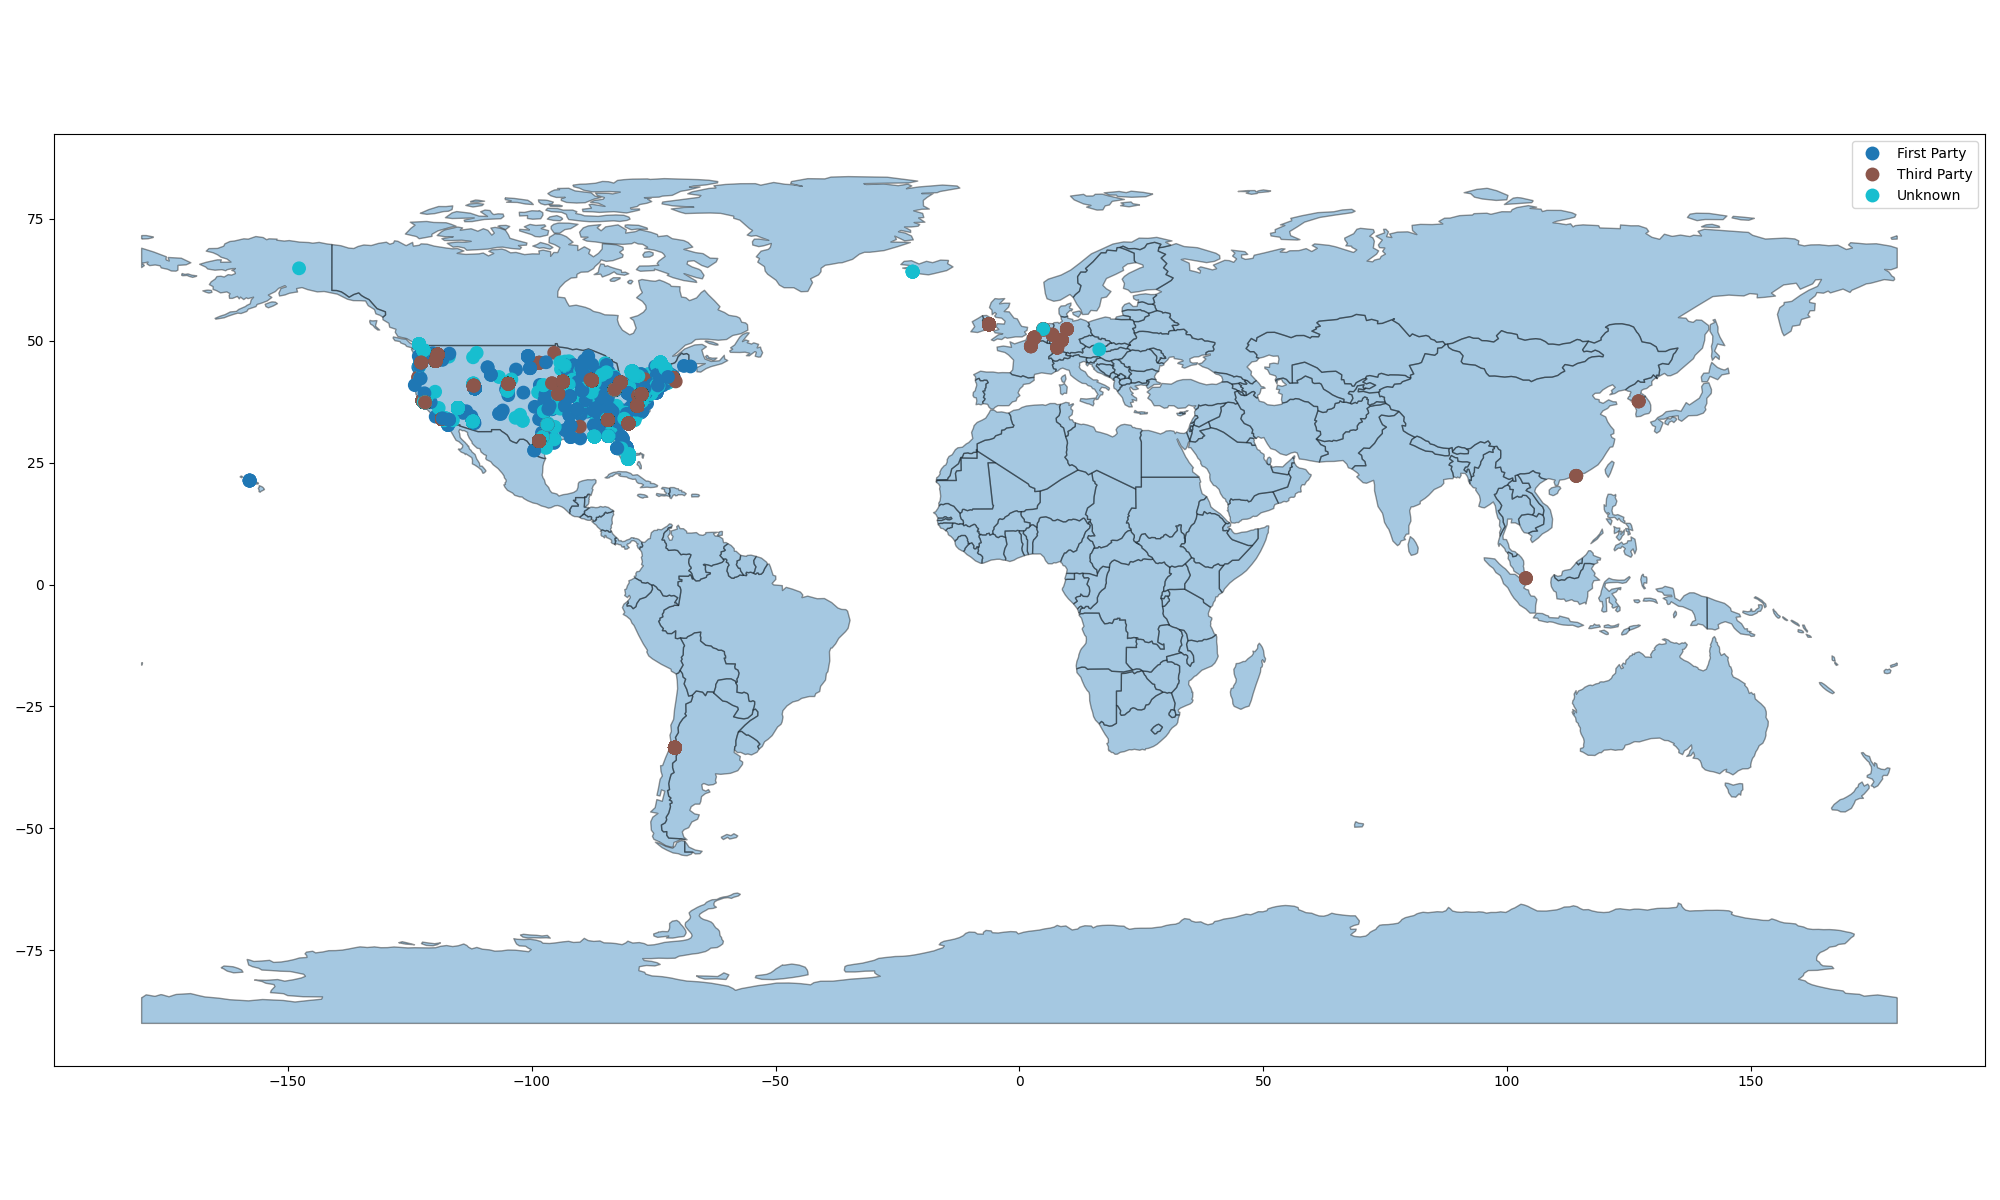
\includegraphics[width=0.5\textwidth]{Summary/Globe Third Party.png}
\caption{First and Third Party Mail Server Locations}
\end{figure}

This lines up with our previous observation that foreign locations are mostly hosted by lower levels of government, at the city, county, and state level, and much less common for federal branches.
We find that 89\% of city, 85\% of county, and 84\% of state mail servers are third party hosted.
Whereas only 31\% of federal legistative 64\% of federal judicial, and 56\% of federal executive servers are third party.
This captures sharply different practices between the upper and lower levels of the US government when it comes to managing server infrastructure.

\section{Limitations}

Our results revolve heavily around IPInfo’s geolocation service, which means that any inaccuracy in the part of IPInfo influences our findings as well.
As mentioned before, the influence of IP Anycast is also something that we fail to account for, meaning that our count of mail servers in a single location is actually a lower bound to the true count.
Finally, using the preference fields for MX records for preference analysis leaves a degree of ambiguity, as we cannot tell whether a domain puts a primary server and multiple backup servers, or whether a domain load balances equally among the servers.

\section{Future Works}

While this study is a strong step towards better understanding of the geolocation of government mail servers, there are nonetheless further avenues for a more robust understanding of the geography of domain, IP, and mailserver distribution.
Most notably is a longitudinal expansion into analyzing the geo locations of mail servers beyond the officially-listed \dotgov domains.
This would include the analysis of the domains of other governments, as well as non-government entities.
Afterall, concern for security is not limited to public services, as other major firms such as Microsoft, Google, Vanguard, etc. all hold sensitive information that could be transmitted across the email architecture.

Furthermore, a thorough analysis of the mail servers themselves beyond geolocation could provide insight beyond physical security into the relevant cyber security of mail servers.
This could be done by applying the methodology outlined in~\cite{bartoli}~in the case of ROA protection.
Only through considered evaluation of both physical and cyber security could the modern email system be adequately secure.

Beyond mail servers, accurate country-level geolocation of critical virtual services should be assessed.
This includes major databases and other infrastructure backing the modern internet.
As technology and the Internet continues to evolve and change, it is vital to continuously curate and understand the relationship between our physical world and the virtual one to ensure that our private and sensitive information remains private.

\section{Conclusion}

In this paper, we analyzed the physical trustworthiness of government mail servers by identifying the geolocation of the servers as well as seeing if the physical server belonged to a third party.
By geolocating the IPs of the mail servers, we found that the servers used were very physically redundant, with 69\% of domains being hosted in 2 or more locations.
Notably, 85\% of mail servers belonged to 2 or less ASes, which impacts AS level redundancy of mail servers.
We also found that there were foreign mail servers as well, all of which belonged to state level government services.
By analyzing the third-party usage of mail servers, we found extensive usage of third party resources, particularly in foreign countries.
Finally, we outlined the procedures we followed to get reliable results, with source code available in a public Github repository in the references below.

\bibliographystyle{abbrv} 
\begin{small}
\bibliography{hotnets21}
\end{small}

\end{document}

